\begin{minipage}[t]{0.495\textwidth}
\centering
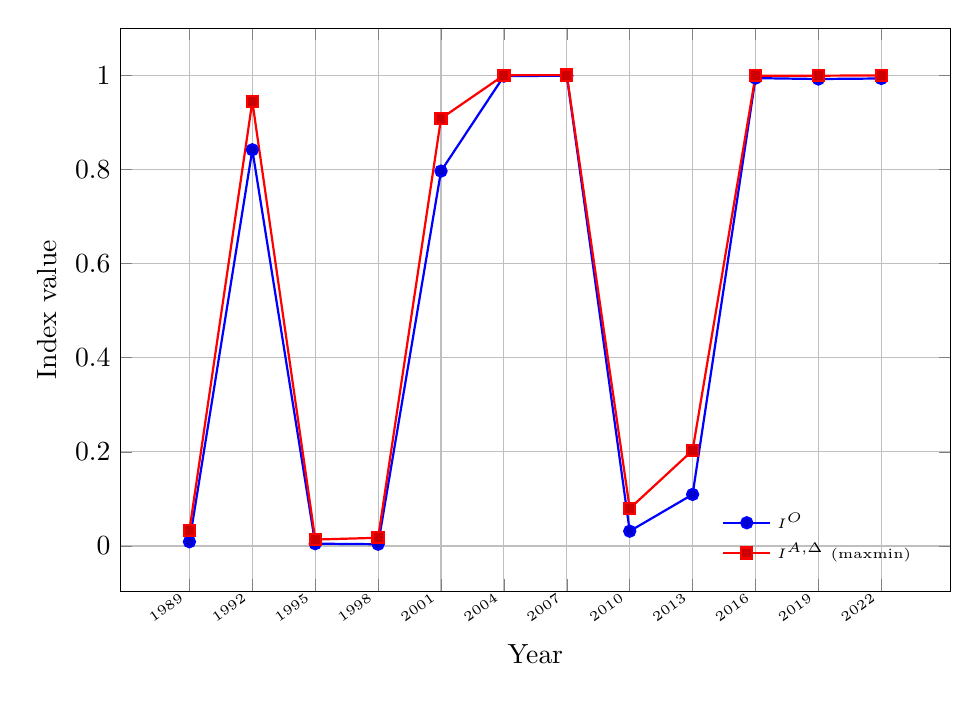
\begin{tikzpicture}
\begin{axis}[
width=\textwidth,
height=0.72\textwidth,
xlabel={Year},
ylabel={Index value},
legend pos=south east,
legend style={font=\tiny,draw=none,fill=none,cells={anchor=west}},
grid=major,
scaled x ticks=false,
xtick={1989,1992,1995,1998,2001,2004,2007,2010,2013,2016,2019,2022},
xticklabel style={/pgf/number format/fixed,/pgf/number format/precision=0,/pgf/number format/1000 sep={},rotate=35,anchor=east,font=\tiny},
]
\addplot+[thick, blue] coordinates {(1989, 0.00889444) (1992, 0.84140353) (1995, 0.00481119) (1998, 0.00368443) (2001, 0.79611426) (2004, 0.99787750) (2007, 0.99858678) (2010, 0.03137790) (2013, 0.10942656) (2016, 0.99353364) (2019, 0.99163267) (2022, 0.99275327)};
\addlegendentry{$I^{O}$}
\addplot+[thick, red] coordinates {(1989, 0.03341930) (1992, 0.94399323) (1995, 0.01359191) (1998, 0.01736261) (2001, 0.90776223) (2004, 0.99985788) (2007, 0.99988502) (2010, 0.07945219) (2013, 0.20298123) (2016, 0.99860221) (2019, 0.99871242) (2022, 0.99919195)};
\addlegendentry{$I^{A,\Delta}$ (maxmin)}
\end{axis}
\end{tikzpicture}
\end{minipage}
\hfill
\begin{minipage}[t]{0.495\textwidth}
\centering
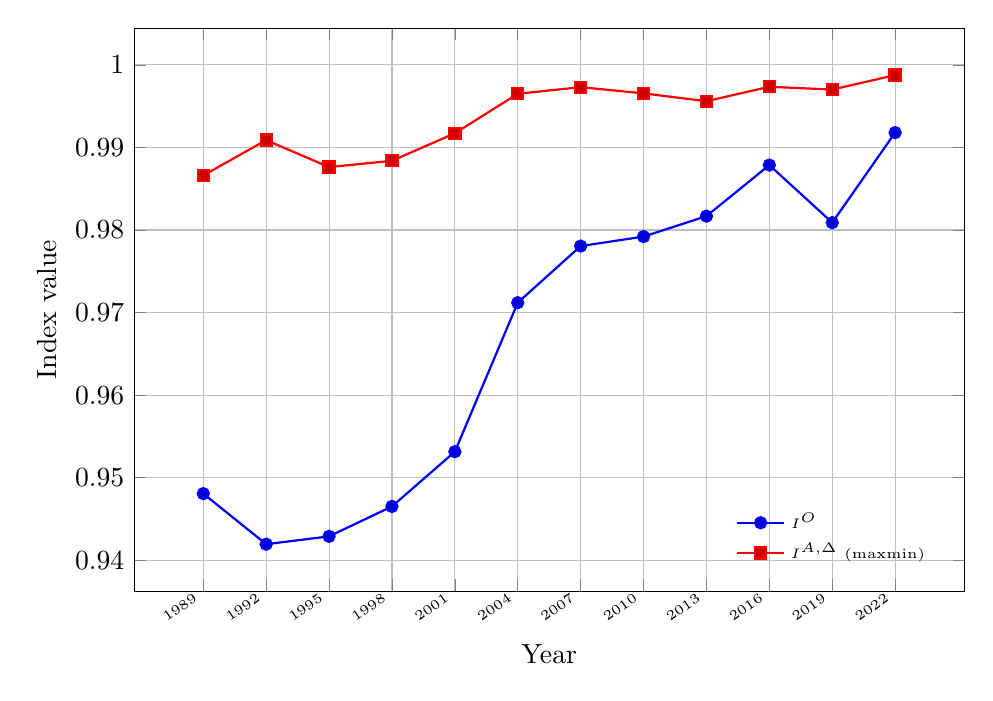
\begin{tikzpicture}
\begin{axis}[
width=\textwidth,
height=0.72\textwidth,
xlabel={Year},
ylabel={Index value},
legend pos=south east,
legend style={font=\tiny,draw=none,fill=none,cells={anchor=west}},
grid=major,
scaled x ticks=false,
xtick={1989,1992,1995,1998,2001,2004,2007,2010,2013,2016,2019,2022},
xticklabel style={/pgf/number format/fixed,/pgf/number format/precision=0,/pgf/number format/1000 sep={},rotate=35,anchor=east,font=\tiny},
]
\addplot+[thick, blue] coordinates {(1989, 0.94807874) (1992, 0.94195748) (1995, 0.94290910) (1998, 0.94652972) (2001, 0.95316151) (2004, 0.97119846) (2007, 0.97805426) (2010, 0.97919781) (2013, 0.98167701) (2016, 0.98785891) (2019, 0.98088954) (2022, 0.99178921)};
\addlegendentry{$I^{O}$}
\addplot+[thick, red] coordinates {(1989, 0.98660459) (1992, 0.99087781) (1995, 0.98761432) (1998, 0.98837475) (2001, 0.99170956) (2004, 0.99649021) (2007, 0.99729218) (2010, 0.99653733) (2013, 0.99559173) (2016, 0.99734023) (2019, 0.99700002) (2022, 0.99874783)};
\addlegendentry{$I^{A,\Delta}$ (maxmin)}
\end{axis}
\end{tikzpicture}
\end{minipage}

{\footnotesize $I^{A,\pi}$ with singleton $C=\{\pi_t\}$ equals $I^{O}$ (audit CSV: columns I\_O and I\_A\_singleton).}

% Gross Assets inequality measures
